\documentclass[conference,10pt]{IEEEtran}
\IEEEoverridecommandlockouts
\usepackage[T1]{fontenc}
\usepackage{cite}
\usepackage{amsmath,amssymb,amsfonts}
\usepackage{algorithm}
\usepackage{algpseudocode}
\usepackage{graphicx}
\usepackage{booktabs}
\usepackage{multirow}
\usepackage{xcolor}
\usepackage{enumitem}
\usepackage{tikz}
\usetikzlibrary{positioning,arrows.meta,fit,backgrounds,calc}
\usepackage[hidelinks]{hyperref}
\graphicspath{{../figures/}}
\renewcommand{\algorithmicrequire}{\textbf{Input:}}
% primitive (expandable) input, so table bodies can sit between booktabs rules
\makeatletter\newcommand{\tabinput}[1]{\@@input #1 }\makeatother

\begin{document}

\title{Future Directions: Integrating Generative AI with Traditional Big Data Pipelines\\[2pt]
\large CONVERGE---Validation-Guided Language-Model Recommendations for Spark Data Cleaning}

\author{\IEEEauthorblockN{Divyanshi Vashistha}
\IEEEauthorblockA{\textit{[Department / Institution]}\\
\textit{[City, Country]}\\
divyanshivashistha@gmail.com}}

\maketitle

\begin{abstract}
Generative language models can supply the semantic judgement that rule-based data cleaning lacks, but wiring their output directly into a big data engine turns every hallucination into a silent, scaled corruption of data. We present \textbf{CONVERGE}, a validation-guided architecture for integrating language models into Apache Spark pipelines in which \emph{AI recommends, a deterministic validator decides, and Spark executes}. The model sees only a bounded, Spark-computed evidence bundle and may only emit typed recommendations from a closed operation catalog; an independent validator cross-checks every recommendation against the same evidence before an immutable, fail-fast plan is executed. We evaluate CONVERGE against a deterministic Spark-only baseline and an unvalidated AI-only pipeline on six controlled-corruption scenarios with per-cell ground truth, using a locally deployed 3B-parameter model (Qwen2.5-Coder) on commodity hardware (54 end-to-end runs), a twelve-class hallucination-injection study, and a scalability study from $10^2$ to $10^6$ rows. AI is necessary for semantic repairs (date-format recall $0\to1$), but unvalidated AI also fabricated issues and modified up to 45 clean cells in a run---damage that conventional before/after quality checks reported as complete success. The validation boundary reduced collateral damage by 71--88\%, rejected nine of eleven checkable hallucination classes (preventing deleted records, smuggled parameters and run aborts), and cost under one millisecond per plan with a prompt size independent of data volume. A recommendation-level audit also exposes the limits of validation: evidentially consistent but semantically wrong repairs, catalog-level evidence conflation, and an evidence-ambiguity defect, each of which we characterise and for which we propose concrete remedies and future research directions.
\end{abstract}

\begin{IEEEkeywords}
big data pipelines, Apache Spark, generative AI, large language models, data cleaning, hallucination, validation, data quality, AI safety
\end{IEEEkeywords}

%======================================================================
\section{Introduction}
\label{sec:intro}
%======================================================================
Spark jobs are trusted because they are boring. A transformation written against the DataFrame API does the same thing on every run, its logical plan can be inspected before execution, and a failed stage can be retried without changing the result~\cite{zaharia2012rdd,zaharia2016spark,armbrust2015sparksql}. Data cleaning has always sat awkwardly inside this model. Removing exact duplicates or trimming whitespace is mechanical, but deciding that \texttt{ENGINEERING} and \texttt{engineering} denote the same department, that \texttt{15/01/2022} should be rewritten as \texttt{2022-01-15}, or that a missing salary should be imputed at all, requires judgement about what the data means. In practice that judgement is either hard-coded as rules or left to an analyst~\cite{rahm2000cleaning,chu2016cleaning,ilyas2019cleaning}.

Large language models (LLMs) can supply some of this judgement from a short description of a column~\cite{narayan2022foundation,zhang2023preprocessors}. The difficulty is what happens when they are wrong. A model that proposes a plausible but unsupported repair, refers to a column that does not exist, or misreads a statistic~\cite{ji2023hallucination,huang2025hallucination} produces exactly the kind of error that a pipeline cannot detect after the fact: the job succeeds, the output has the right schema, and the damage is spread across millions of rows. Integration patterns that let a model write and run code, such as text-to-SQL and tool-calling agents~\cite{rajkumar2022texttosql,li2023bird,yao2023react,schick2023toolformer}, make this failure mode easier to reach.

This paper evaluates one answer to the question in its title. CONVERGE is a pipeline in which the model is allowed to \emph{recommend} cleaning operations but never to execute them. The model receives a bounded summary of the data computed by Spark and returns typed recommendations drawn from a closed catalog of eight operations. A deterministic validator, which has no dependency on the model, re-reads the same Spark evidence and decides which recommendations may run. Spark then executes the approved plan unchanged and refuses to publish partial output.

We compare this design with two alternatives that share every other component: a Spark-only baseline that applies the two repairs the evidence fully determines, and an \textsc{AI\_Only} pipeline that executes the same model's recommendations after a structural filter. Because the profiler, prompt, executor and evaluator are identical across the three arms, differences in outcome are attributable to the decision layer.

The study makes five contributions.
\begin{enumerate}[leftmargin=*,nosep]
  \item An architecture for model-assisted cleaning in Spark with five stated safety properties, implemented as a ten-state auditable pipeline (\S\ref{sec:problem}, \S\ref{sec:arch}).
  \item A controlled-corruption benchmark with per-cell ground truth and metrics that separate repair quality, collateral damage and run availability from the data-quality signals a pipeline normally observes (\S\ref{sec:method}).
  \item An end-to-end evaluation with a locally served 3B-parameter model across six scenarios and three corruption seeds, with bootstrap intervals and paired permutation tests (\S\ref{sec:res-e1}, \S\ref{sec:res-seeds}).
  \item A record-and-replay methodology that re-runs the model's actual outputs through fifteen decision pipelines, giving paired, causal estimates of what each validator rule contributes and evaluating three defect fixes and two new semantic guards on held-out seeds (\S\ref{sec:res-replay}).
  \item A twelve-class hallucination taxonomy with an injection study, a token-level cost analysis, and a scalability study to $10^6$ rows, which together locate precisely what validation can and cannot prevent (\S\ref{sec:res-inject}, \S\ref{sec:res-scale}).
\end{enumerate}

The headline result is mixed in an informative way. The model was necessary for one class of repair (date formats, recall $0\to1$) and harmful for another: on the missing-value and categorical scenarios it invented problems and rewrote correct values, and the comparator that a pipeline would normally use to judge cleaning reported those runs as complete successes. The shipped validator removed most of that damage, but the replay study shows that part of its apparent success came from a defect, and that two small deterministic guards are needed before the design behaves as intended on unseen data.

%======================================================================
\section{Background and Related Work}
\label{sec:related}
%======================================================================
\subsection{Data Cleaning at Scale}
Classical cleaning separates error detection from repair~\cite{rahm2000cleaning,chu2016cleaning,ilyas2019cleaning,hellerstein2008quantitative}. Constraint-based approaches such as conditional functional dependencies~\cite{fan2008cfd} give repairs a formal meaning but need curated rules. HoloClean~\cite{rekatsinas2017holoclean} combines constraints, statistics and external signals in a probabilistic model; ActiveClean~\cite{krishnan2016activeclean} and Raha~\cite{mahdavi2019raha} reduce the human effort needed to configure detection. Abedjan et al.~\cite{abedjan2016detecting} found that no single detector dominates across real datasets. Closer to pipeline engineering, Deequ~\cite{schelter2018deequ} expresses data-quality checks as Spark computations, and TFX data validation~\cite{breck2019validation} checks training data against a schema before it reaches a model. CONVERGE borrows the second idea, deterministic checks computed by the engine itself, but applies it to \emph{proposed actions} rather than to the data alone.

\subsection{Language Models for Data Preparation}
Narayan et al.~\cite{narayan2022foundation} showed that foundation models can match specialised systems on entity matching, imputation and error detection with few examples, and Zhang et al.~\cite{zhang2023preprocessors} reported similar results for a range of preprocessing tasks. Earlier, Wrangler~\cite{kandel2011wrangler} established the value of \emph{suggesting} transformations to a user rather than applying them. These studies measure whether the model's answer is right. They do not ask what a pipeline should do when it is wrong, which is the question for any unattended deployment. Text-to-SQL benchmarks~\cite{rajkumar2022texttosql,li2023bird} and agent frameworks~\cite{yao2023react,schick2023toolformer,shinn2023reflexion} go further by executing model output; our \textsc{AI\_Only} arm reproduces that pattern under a restricted action space.

\subsection{Hallucination and Guarding Model Output}
Surveys of hallucination~\cite{ji2023hallucination,huang2025hallucination} distinguish errors that contradict the input from errors that contradict the world. Retrieval augmentation~\cite{lewis2020rag} targets the second; constrained decoding~\cite{willard2023outlines} guarantees that output is syntactically valid but says nothing about whether it is true. Indirect prompt injection~\cite{greshake2023injection} shows that anything the model reads can carry instructions, which matters here because evidence contains raw cell values. From a security standpoint, Saltzer and Schroeder's principles of least privilege and complete mediation~\cite{saltzer1975protection} argue that an untrusted component should hold no execution authority and that every request it makes should be checked. CONVERGE applies these principles literally: the model can only propose, and every proposal passes through a validator that does not depend on the model.

\subsection{Positioning}
Existing work either cleans deterministically without semantic judgement or uses models for judgement without an execution boundary. We are not aware of a study that measures, against per-cell ground truth, how an evidence-based validation boundary changes the outcome of model-driven cleaning, or one that decomposes that change rule by rule on the model's own outputs.

%======================================================================
\section{Problem Formulation and Threat Model}
\label{sec:problem}
%======================================================================
Let $D$ be a table with columns $C=\{c_1,\dots,c_m\}$ and $n$ rows. The Spark profiler computes $\pi(D)=(P,E)$, where $P$ holds per-column statistics (physical and semantic type, null and distinct counts, quantiles, date-pattern histograms) and $E=\{e_1,\dots,e_k\}$ is a set of evidence items. Each $e=(\tau,C_e,\sigma)$ names an issue type $\tau$ (missing values, duplicates, categorical inconsistency, whitespace, date-format inconsistency, outlier candidate), a column set $C_e\subseteq C$, and bounded supporting data $\sigma$ such as a variant histogram. The sizes of $E$ and $\sigma$ are capped by configuration, not by $n$.

The operation catalog $\mathcal{O}$ assigns each permitted operation $o$ a safety tier $t(o)\in\{\textsc{safe},\textsc{review},\textsc{finding}\}$, compatible semantic types $S(o)$, a parameter schema $\Theta(o)$ and required evidence types $R(o)$. A separate set $\mathcal{F}$ of forbidden names (e.g., \texttt{DELETE\_COLUMN}, \texttt{ARBITRARY\_CODE}, \texttt{JOIN}) is recognised and always refused.

The model $M$ maps $(P,E,\mathcal{O})$ to recommendations $r=(o,C_r,\theta,\rho,\mathrm{refs})$: an operation, target columns, parameters, a free-text reason, and evidence references with \emph{claimed values}. We treat every field of $r$ as untrusted.

\noindent\textbf{Checkable hallucinations.} A recommendation is hallucinated if it violates any of the following: (H-op) $o\in\mathcal{O}\setminus\mathcal{F}$; (H-col) $C_r\subseteq C$; (H-type) every $c\in C_r$ has $\mathrm{sem}(c)\in S(o)$; (H-param) $\theta$ conforms to $\Theta(o)$ with no extra keys; (H-evid) some $e\in E$ has $\tau_e\in R(o)$ and covers $C_r$ (with equality for row-level operations); (H-claim) each claimed value equals the corresponding entry of $\sigma$; (H-value) each raw value named in $\theta$ occurs in $\sigma$. These predicates can be evaluated from $(P,E)$ alone. A recommendation can also be \emph{semantically wrong} while satisfying all of them, for instance by mapping a genuine variant of ``Marketing'' to ``Sales''. Part of our evaluation asks how much of this second class can be recovered by additional predicates that are still computable from evidence (\S\ref{sec:res-replay}).

\noindent\textbf{Safety properties.} The design aims to guarantee:
\begin{enumerate}[label=\textbf{P\arabic*},leftmargin=*,nosep]
  \item \emph{Bounded exposure}: $M$ observes only $(P,E,\mathcal{O})$; never rows, file paths or engine handles.
  \item \emph{Closed action space}: outputs are typed data, and no field is evaluated as code.
  \item \emph{Complete mediation}: no $r$ is executed unless the validator returns an executable status.
  \item \emph{Monotone approval}: an approval policy can narrow the validator's verdicts but not widen them.
  \item \emph{Immutable, fail-fast execution}: the executor applies a frozen plan in order, re-checks parameters, and writes nothing if any operation fails.
\end{enumerate}
The threat model is a model that is mistaken rather than adversarial, although P1--P3 also bound the effect of injected instructions carried in cell values.

%======================================================================
\section{The CONVERGE Architecture}
\label{sec:arch}
%======================================================================
Fig.~\ref{fig:arch} shows the end-to-end architecture. Its organising principle is a strict separation of \emph{authority}: Spark is authoritative for facts, the LLM is authoritative for nothing, the validator is authoritative for admissibility, and the approval boundary is authoritative for consent.

\begin{figure*}[t]
\centering
\resizebox{\textwidth}{!}{%
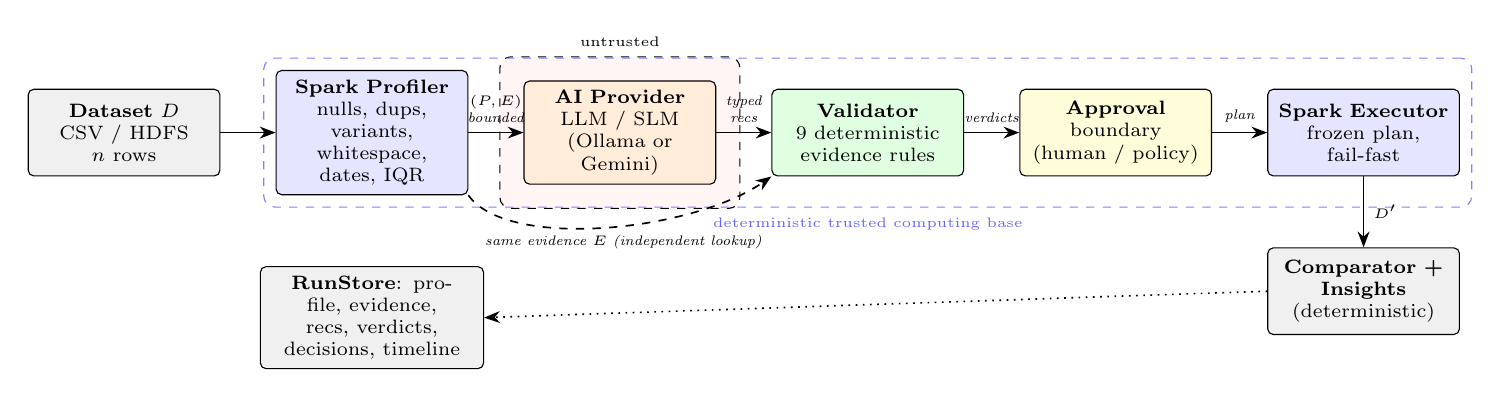
\begin{tikzpicture}[
  node distance=4mm and 7mm,
  box/.style={draw, rounded corners=2pt, minimum height=11mm, text width=22mm, align=center, font=\scriptsize, fill=#1},
  box/.default=white,
  lab/.style={font=\tiny\itshape, align=center},
  arr/.style={-{Stealth[length=2mm]}, semithick},
  trust/.style={draw, dashed, rounded corners=4pt, inner sep=3mm}]
\node[box=gray!12] (data) {\textbf{Dataset} $D$\\ CSV / HDFS\\ $n$ rows};
\node[box=blue!10, right=of data] (prof) {\textbf{Spark Profiler}\\ nulls, dups, variants,\\ whitespace, dates, IQR};
\node[box=orange!15, right=of prof] (ai) {\textbf{AI Provider}\\ LLM / SLM\\ (Ollama or Gemini)};
\node[box=green!12, right=of ai] (val) {\textbf{Validator}\\ 9 deterministic\\ evidence rules};
\node[box=yellow!15, right=of val] (appr) {\textbf{Approval}\\ boundary\\ (human / policy)};
\node[box=blue!10, right=of appr] (exec) {\textbf{Spark Executor}\\ frozen plan,\\ fail-fast};
\node[box=gray!12, below=9mm of exec] (cmp) {\textbf{Comparator +}\\ \textbf{Insights}\\ (deterministic)};
\node[box=gray!12, below=9mm of prof, text width=26mm] (store) {\textbf{RunStore}: profile, evidence, recs, verdicts, decisions, timeline};
\draw[arr] (data) -- (prof);
\draw[arr] (prof) -- node[lab, above]{$(P,E)$\\bounded} (ai);
\draw[arr] (ai) -- node[lab, above]{typed\\recs} (val);
\draw[arr] (val) -- node[lab, above]{verdicts} (appr);
\draw[arr] (appr) -- node[lab, above]{plan} (exec);
\draw[arr] (exec) -- node[lab, right]{$D'$} (cmp);
\draw[arr, dashed] (prof.south east) .. controls +(0.5,-0.7) and +(-1.0,-0.7) .. node[lab, below, pos=0.55]{same evidence $E$ (independent lookup)} (val.south west);
\draw[arr, dotted] (cmp.west) -- (store.east);
\begin{scope}[on background layer]
\node[trust, fit=(ai), fill=red!4, label={[font=\tiny]above:untrusted}] {};
\node[trust, fit=(prof)(val)(exec), draw=blue!50, label={[font=\tiny, blue!60]below:deterministic trusted computing base}, inner sep=1.5mm] {};
\end{scope}
\end{tikzpicture}}
\caption{CONVERGE architecture. The language model (red, untrusted) sees only the bounded profile/evidence $(P,E)$ and emits typed recommendations. The validator independently re-reads the \emph{same} Spark evidence; only admissible, approved recommendations become an immutable execution plan. Measurement is deterministic and external to the AI.}
\label{fig:arch}
\end{figure*}

\subsection{Spark Profiler and Bounded Evidence}
The profiler (\texttt{services/spark/profiler.py}) is the only component that reads $D$. For each column it classifies a \emph{semantic type} (integer, float, string, date-like string, boolean) separately from the physical Spark dtype, computes null statistics, distinct counts, IQR outlier bounds, case/whitespace-normalised \emph{variant groups} for categorical columns, and a histogram of detected date patterns. Identifier-like columns (an \texttt{id} name pattern and $\geq90\%$ distinct values) are excluded from duplicate criteria. From the profile, it emits one evidence item per detected issue; nothing is fabricated for absent issues. Evidence carries only issue-scoped raw values---e.g., the variant histogram $\{\texttt{Engineering}{:}5,\texttt{engineering}{:}1,\texttt{ENGINEERING}{:}1\}$---capped by \texttt{MAX\_EVIDENCE\_DISTINCT\_VALUES}$=30$ and \texttt{MAX\_EVIDENCE\_SAMPLE\_ROWS}$=10$. Before prompting, the prompt builder additionally \emph{redacts} unscoped raw fields (per-column samples and top-value lists), so that, for example, personal names in an unflagged column are never sent to the model. This realises P1 and has a second, decisive consequence: the prompt size is $O(m+|E|)$ and independent of $n$ (verified in \S\ref{sec:res-scale}).

\subsection{Operation Catalog and Safety Tiers}
Table~\ref{tab:catalog} lists the eight P0 operations. Operations are declarative, parameterised, and implemented exclusively with the Spark DataFrame API---no \texttt{spark.sql()}, \texttt{eval}, or dynamic dispatch on parameter content. The \textsc{safe} tier covers value-preserving normalisations; \textsc{review} covers operations that synthesise values or change row counts and are capped at \textsc{needs\_review} regardless of evidence; \textsc{finding} operations can never execute. The same registry generates the prompt's operation list, the validator's rules, and the traceability map, so the three cannot drift apart (ADR-002).

\begin{table}[t]
\centering
\caption{Operation catalog (P0). Tier caps the best achievable verdict.}
\label{tab:catalog}
\scriptsize
\setlength{\tabcolsep}{3pt}
\resizebox{\columnwidth}{!}{%
\begin{tabular}{@{}llll@{}}
\toprule
\textbf{Operation} & \textbf{Tier} & \textbf{Parameters} & \textbf{Required evidence}\\
\midrule
\texttt{TRIM\_WHITESPACE} & safe & -- & whitespace\\
\texttt{NORMALIZE\_CASE} & safe & case$\in$\{lower,upper,title\} & categorical $\lor$ ws\\
\texttt{STANDARDIZE\_CATEGORY} & safe & mapping: raw$\to$canonical & categorical\\
\texttt{STANDARDIZE\_DATE\_FORMAT} & safe & fmt$\in$\{ISO, D/M/Y, M/D/Y\} & date-format\\
\texttt{FILL\_MISSING} & review & mean$|$median$|$mode$|$const & missing\\
\texttt{CONVERT\_DTYPE} & review & int$|$float$|$str$|$bool & --\\
\texttt{REMOVE\_DUPLICATES} & review & criteria $=$ target cols & duplicates (exact)\\
\texttt{FLAG\_OUTLIER} & finding & -- & outlier\\
\midrule
\multicolumn{4}{@{}l}{\textit{Forbidden:} \texttt{DELETE\_COLUMN, DELETE\_DATASET, JOIN, PIVOT, MERGE,}}\\
\multicolumn{4}{@{}l}{\quad\texttt{ARBITRARY\_ROW\_FILTER, ARBITRARY\_CODE, SCHEMA\_RESTRUCTURING}}\\
\bottomrule
\end{tabular}}
\end{table}

\subsection{AI Provider and Prompt Contract}
Providers implement a four-member interface: \texttt{provider\_name}, \texttt{model\_name}, \texttt{prompt\_version}, and \texttt{generate\_\allowbreak{}recommendations(\allowbreak{}ProfileResult)} $\to$ \texttt{list[\allowbreak{}Recommendation]}. The signature itself enforces P1 and P2: there is no parameter through which raw data could enter and no return channel for code. Two implementations exist: a remote Gemini provider~\cite{gemini2023} using native response-schema enforcement, and a local Ollama provider using JSON-schema-constrained decoding~\cite{willard2023outlines} at temperature $0$. Both share one versioned system prompt (\texttt{recommendation-prompt-v1}) stating eight rules: Spark evidence is authoritative; do not invent facts; do not calculate; only use catalog operations; never produce code; never propose destructive operations; cite evidence with checkable claimed values; and return \emph{fewer} recommendations when evidence is insufficient. Output is parsed strictly with Pydantic; any malformed item fails the stage with a typed \texttt{AIProviderResponseError} rather than being silently repaired. Note that \texttt{operation} is deliberately typed as a free string rather than an enum, so that an invented operation \emph{constructs} successfully and is rejected by the validator with an auditable explanation instead of an opaque parse error.

\subsection{Independent Validator}
The validator (Algorithm~\ref{alg:validator}) is constructed once per profile and has no dependency on the AI provider, the executor, or the orchestrator (ADR-003); it can be tested in isolation against hand-built recommendations. Rules are evaluated in order and short-circuit on the first failure, and every check is recorded with a human-readable message, giving a complete audit trail. The evidence rules are the core novelty: they do not trust the model's \texttt{evidence\_refs}, but independently search $E$ for an item of a required type covering the targets. For row-level operations the criteria set must equal the profiler's criteria \emph{exactly}, preventing the model from asserting duplicate support for a column set Spark never verified. Claimed numeric values are compared with tolerance $10^{-6}$, and every raw key of a category mapping must occur in the evidence's variant histogram.

\begin{algorithm}[t]
\caption{Evidence-based validation $V(r;P,E)$}
\label{alg:validator}
\footnotesize
\begin{algorithmic}[1]
\Require recommendation $r=(o,C_r,\theta,\cdot,\mathrm{refs})$; profile $P$; evidence $E$
\If{$o\in\mathcal{F}$ \textbf{or} $o\notin\mathcal{O}$} \Return \textsc{rejected} \Comment{R1, R8}\EndIf
\If{$C_r=\emptyset$ \textbf{or} $C_r\not\subseteq C$} \Return \textsc{rejected} \Comment{R2}\EndIf
\If{$\neg\mathrm{rowlevel}(o)\wedge\exists c\in C_r:\mathrm{sem}(c)\notin S(o)$} \Return \textsc{rejected}\EndIf
\If{$\theta$ has unknown keys, missing/ill-typed required keys, or values $\notin$ allowed} \Return \textsc{rejected}\EndIf
\If{$R(o)\neq\emptyset$}
  \State $M\gets\{e\in E:\tau_e\in R(o)\wedge(\mathrm{rowlevel}(o)\,?\,C_e{=}C_r : C_r{\subseteq}C_e)\}$
  \If{$M=\emptyset$} \Return \textsc{rejected} \Comment{R6: no Spark evidence}\EndIf
  \ForAll{$(k,v)\in\mathrm{refs}.\mathrm{claimed}$ with $k\in\sigma_e$, $e\in M$}
    \If{$|v-\sigma_e[k]|>\epsilon$} \Return \textsc{rejected} \Comment{R7}\EndIf
  \EndFor
  \If{$o=\texttt{STANDARDIZE\_CATEGORY}\wedge\mathrm{keys}(\theta.\mathrm{map})\not\subseteq\bigcup_{e\in M}\mathrm{variants}(e)$} \Return \textsc{rejected}\EndIf
\EndIf
\If{$t(o)=\textsc{finding}$} \Return \textsc{not\_executable}\EndIf
\State \Return $t(o)=\textsc{safe}\ ?\ \textsc{approved\_auto} : \textsc{needs\_review}$
\end{algorithmic}
\end{algorithm}

\subsection{Approval Boundary and Pipeline State Machine}
The orchestrator drives an explicit state machine: \textsc{ingested} $\to$\allowbreak{} \textsc{profiled} $\to$\allowbreak{} \textsc{ai\_analyzed} $\to$\allowbreak{} \textsc{validated} $\to$\allowbreak{} \textsc{awaiting\_approval} $\to$\allowbreak{} \textsc{executing} $\to$\allowbreak{} \textsc{cleaned} $\to$\allowbreak{} \textsc{stats\_computed} $\to$\allowbreak{} \textsc{insights\_generated} $\to$\allowbreak{} \textsc{completed}, with \textsc{failed} reachable from any stage. Every transition is timestamped and persisted. The pipeline \emph{hard-pauses} at \textsc{awaiting\_approval}; nothing executes without an explicit decision per recommendation. In interactive use a human approves \textsc{needs\_review} items; in experiments a documented policy approves exactly what the validator deemed executable. P4 is enforced twice: \texttt{submit\_decision} raises \texttt{RecommendationNotEligibleError} for an ineligible approval, and the experiment adapter ANDs any policy with the validator's verdict so a misconfigured policy fails safe.

\subsection{Spark Executor}
Approved recommendations are compiled into a frozen \texttt{ExecutionPlan}, ordered by a fixed technical precedence (dtype conversion $\to$ imputation $\to$ text/category normalisation $\to$ date formatting $\to$ deduplication) so that, e.g., trimming precedes duplicate detection. The executor applies operations exactly in plan order, re-checks every parameter (defence in depth), counts affected rows, and on the first failure marks remaining operations \textsc{skipped} and writes no output (P5). Partial cleaning is never published.

\subsection{Deterministic Comparison and Insights}
After execution the cleaned dataset is re-profiled with the \emph{same} profiler and compared per issue as \emph{resolved}, \emph{improved}, \emph{unchanged}, \emph{worsened}, or \emph{introduced}. A traceability map links each executed recommendation to the issues it targeted, and a deterministic insight generator summarises outcomes in templated natural language. No model is consulted after execution: the system never asks the AI to grade its own work (ADR-007, ADR-009).

\subsection{Design Rationale}
Three design decisions merit justification. \emph{(i) Recommendation, not generation of code.} Generating Spark or SQL code would give the model an unbounded action space; restricting it to a catalog makes every possible action enumerable, testable, and reviewable. \emph{(ii) Validation against evidence, not against the model's claims.} Self-consistency checks on model output are vulnerable to correlated errors; checking against an independent deterministic artefact breaks that correlation. \emph{(iii) A narrow deterministic baseline.} The \textsc{Spark\_Only} arm applies only the two remediations whose correct action is fully determined by evidence (trim whitespace; drop profiler-verified duplicates), and \emph{refuses} to invent heuristics (e.g., ``most frequent variant is canonical'') for the rest. Determinism is not correctness; the baseline therefore marks exactly the boundary where semantic judgement---and hence AI---becomes necessary.

%======================================================================
\section{Experimental Methodology}
\label{sec:method}
%======================================================================
\subsection{Research Questions}
\begin{description}[leftmargin=*,nosep,font=\normalfont\bfseries]
  \item[RQ1] Does model-assisted cleaning repair more corruption than a deterministic Spark-only baseline?
  \item[RQ2] Does the validation boundary reduce errors caused by incorrect model output, and what does it cost in lost repairs?
  \item[RQ3] Which validator rules account for the effect, and which failure classes remain?
  \item[RQ4] What do the model call and the control plane cost, and how do they scale with data volume?
\end{description}

\subsection{Arms}
All arms use the same loader, profiler, operation catalog, executor, prompt, model and evaluator (ADR-007); only the decision layer differs.
\textbf{\textsc{Spark\_Only}} applies \texttt{TRIM\_WHITESPACE} to whitespace evidence and \texttt{REMOVE\_DUPLICATES} on profiler-established criteria, and records an explicit reason for skipping every other issue. An import-scanning test enforces that it never loads the AI package.
\textbf{\textsc{AI\_Only}} executes the model's recommendations in the model's order after a structural filter (operation registered and executable, at least one target). An import-scanning test enforces that it never loads the validator. The executor's own parameter checks still apply.
\textbf{\textsc{Converge}} runs the orchestrator with the validator and an approval policy that approves exactly the recommendations the validator marks executable. The adapter stops at \textsc{cleaned} so that no arm grades its own output.

\subsection{Scenarios and Ground Truth}
A 15-row, 7-column employee table (\texttt{\_row\_id}, \texttt{name}, \texttt{department}, \texttt{city}, \texttt{hire\_date}, \texttt{salary}, \texttt{rating}) is corrupted by a seeded generator into six scenarios (Table~\ref{tab:scenarios}). Each injected change is recorded in a manifest with its row, column, clean value and corrupted value, and each scenario file's SHA-256 checksum is verified before every run. The table is deliberately small so that every cell can be audited; volume is studied separately in E3.

\begin{table}[t]
\centering
\caption{Controlled corruption scenarios (examples from seed 42).}
\label{tab:scenarios}
\scriptsize
\begin{tabular}{@{}llrl@{}}
\toprule
\textbf{ID} & \textbf{Corruption} & \textbf{\#} & \textbf{Target / example}\\
\midrule
S1 & Whitespace injection & 3 & \texttt{name}: ``\verb*|  Alice Martin  |''\\
S2 & Exact duplicate rows & 2 & whole row, new \texttt{\_row\_id}\\
S3 & Categorical case variants & 3 & \texttt{department}: ``\texttt{mARKETING}''\\
S4 & Missing values & 2 & \texttt{salary}: empty\\
S5 & Mixed date formats & 3 & \texttt{hire\_date}: ``\texttt{15/01/2022}''\\
S6 & All five combined & 13 & mixed (3+2+3+2+3)\\
\bottomrule
\end{tabular}
\end{table}

\subsection{Metrics}
Let $\mathcal{K}$ be the injected cell corruptions, $\mathrm{out}(i,c)$ the output value for row $i$ and column $c$ (joined on \texttt{\_row\_id}) and $\mathrm{clean}(i,c)$ the reference value. Comparison is exact, including case and whitespace.
\begin{align}
\text{Recall} &= |\{(i,c)\in\mathcal{K}:\mathrm{out}(i,c)=\mathrm{clean}(i,c)\}|\,/\,|\mathcal{K}|,\\
\text{Damage} &= |\{(i,c)\notin\mathcal{K}:\mathrm{out}(i,c)\neq\mathrm{clean}(i,c)\}| + \text{rows lost}.
\end{align}
A corrupted cell is \emph{incorrectly repaired} when its output matches neither the clean nor the corrupted value. \emph{Rows lost} counts clean-reference rows missing from the output, the most severe form of collateral damage. For S2, which has no cell corruptions, we report the fraction of injected duplicates removed. Repair precision is not reported because a strategy's intended modifications cannot be observed from its output. Separately, we record the comparator's before/after count of detected issues. This is the signal a production pipeline would see, and we keep it apart from correctness (ADR-009). Run availability is the fraction of runs that produce output; an executor fail-fast abort produces none.

\subsection{Model and Platform}
The model is Qwen2.5-Coder 3B~\cite{hui2024qwencoder} (4-bit quantised, 1.9\,GB), served by Ollama 0.34 with JSON-schema-constrained decoding at temperature 0. A small local model represents deployments where data and metadata may not leave the cluster, and it is the setting where structured-output errors are most common. All runs use one laptop (AMD Ryzen 3 5300U, 4 cores/8 threads, 7.5\,GB RAM, no GPU). Spark 3.5.1 runs in \texttt{local[*]} mode on OpenJDK 17 and Python 3.12 in Ubuntu 24.04 under WSL2; Ollama runs on the Windows host, so inference and Spark share the same cores. Experiments were run one at a time.

\subsection{Experiments}
\noindent\textbf{E1, end-to-end matrix.} Six scenarios $\times$ three arms $\times$ three repetitions with seed 42 (54 runs). For every \textsc{Converge} run we reload the persisted pipeline artefact and classify each recommendation by verdict and failing rule.

\noindent\textbf{E4, seed sweep.} S3, S4 and S6, the scenarios that require more than one decision, are regenerated with corruption seeds 7 and 123, which place the corruptions in different rows and draw different variant spellings. With seed 42 this gives 9 runs per (scenario, arm). Every model call is logged with its raw output, token counts and Ollama's prefill and decode timings.

\noindent\textbf{E5, record-and-replay.} The \textsc{AI\_Only} and \textsc{Converge} arms in E1 and E4 make separate model calls, so their comparison mixes the effect of validation with variation in model output. To remove that confound we collect every recommendation list the model produced (18 from E1, 36 from E4) and replay each one, unchanged, through fifteen decision pipelines: \textsc{AI\_Only} with and without CONVERGE's operation precedence; the shipped validator (V0); V0 with each of four modifications; two combinations; and four ablations that disable one rule family. Each distinct (dataset, plan) pair is executed once with the real executor and scored with the same evaluator. Since every pipeline sees identical model output, paired differences between pipelines are causal effects of the decision layer. The modifications were designed after inspecting the seed-42 audit, so we report seed 42 and the held-out seeds 7 and 123 separately.

\noindent\textbf{E2, hallucination injection.} A scripted provider returns an oracle plan built from S6's evidence plus one hallucination from a twelve-class taxonomy, either appended or substituted for its correct counterpart. Each case runs end-to-end through \textsc{AI\_Only} and \textsc{Converge}, and is also replayed through the E5 pipelines.

\noindent\textbf{E3, scalability.} Synthetic tables of $10^2$ to $10^6$ rows with a 10\% mixed corruption rate measure profiling, prompt size, validation and execution separately.

\subsection{Statistical Procedure}
Means are reported with percentile bootstrap 95\% confidence intervals (10{,}000 resamples). Paired comparisons use a two-sided sign-flip permutation test on per-unit differences, exact for $n\le20$ and Monte Carlo ($10^5$ draws) otherwise. In E1/E4 the pairing unit is (seed, repetition); in E5 it is the individual model output, which is a much tighter pairing. With 9 runs per cell in E4 we treat $p$-values as descriptive and do not correct for multiplicity.

%======================================================================
\section{Results}
\label{sec:results}
%======================================================================
All 54 E1 runs completed successfully (success rate $1.00$ for every cell); no provider timeouts or schema-parse failures occurred with constrained decoding. Table~\ref{tab:main} and Fig.~\ref{fig:main} summarise ground-truth outcomes.

\begin{table*}[t]
\centering
\caption{E1 end-to-end results (mean over 3 repetitions; $\pm$ is s.d.). \emph{Recall}: correctly repaired / injected corruptions (S2: fraction of injected duplicates removed). \emph{C/I/U}: correctly repaired, incorrectly repaired, unrepaired cells. \emph{Dmg}: originally clean cells modified. \emph{Issues}: comparator's detected issue count before$\to$after (an observed signal, not correctness). \emph{Time}: strategy wall time in seconds, including the LLM call.}
\label{tab:main}
\footnotesize
\begin{tabular}{@{}llcccccr@{}}
\toprule
\textbf{Scen.} & \textbf{Arm} & \textbf{Recall} & \textbf{C/I/U} & \textbf{Dmg} & \textbf{FMR} & \textbf{Issues} & \textbf{Time}\\
\midrule
\tabinput{../tables/main_results.tex}
\bottomrule
\end{tabular}
\end{table*}

\begin{figure*}[t]
\centering
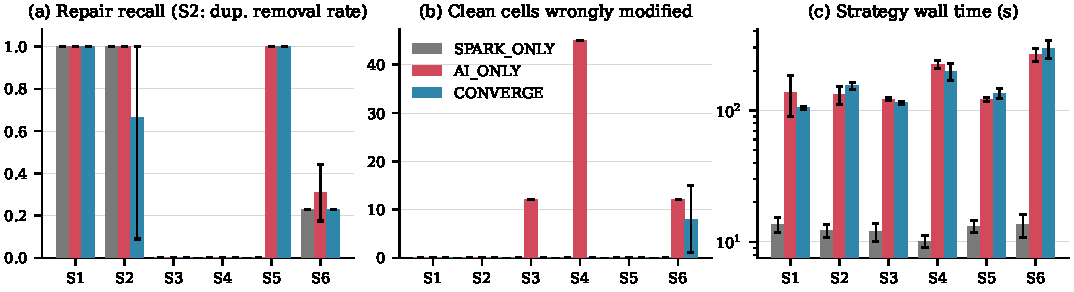
\includegraphics[width=\textwidth]{main_results.pdf}
\caption{E1 results by scenario and arm. (a) Ground-truth repair quality; (b) collateral damage to originally clean cells; (c) strategy wall time (log scale). AI is necessary for date and categorical semantics (S5), but unvalidated AI causes all of the large collateral damage (S3, S4).}
\label{fig:main}
\end{figure*}

\subsection{RQ1: Does AI Improve Repair Quality?}
\label{sec:res-rq1}
\emph{Where the corruption requires a semantic decision and the model makes the right one, yes---decisively.} On S5 (mixed date formats) the deterministic baseline, which by design refuses to choose a target format, leaves all three corrupted dates unrepaired (recall $0.00$), whereas both AI arms choose \texttt{STANDARDIZE\_DATE\_FORMAT} with target \texttt{YYYY-MM-DD} in every repetition and restore all three cells exactly (recall $1.00$, zero collateral damage).

\emph{Where the corruption is mechanically determined, AI adds nothing.} On S1 all three arms reach recall $1.00$; as discussed in \S\ref{sec:discussion}, this is partly an artefact of Spark's CSV writer, which trims whitespace on output, as the no-op control in E2 confirms. On S2 the baseline and \textsc{AI\_Only} both remove both injected duplicates without losing an original row.

\emph{Where the corruption is information-theoretically unrecoverable, no arm succeeds.} On S4 the true salaries cannot be derived from aggregates; \textsc{AI\_Only}'s mean imputation produces two \emph{incorrect} repairs, while \textsc{Spark\_Only} and \textsc{Converge} leave the cells missing.

\emph{Where the model's judgement is wrong, AI makes things worse.} On S3 the model consistently proposed \texttt{NORMALIZE\_CASE(lower)} on \texttt{department} rather than a canonicalising \texttt{STANDARDIZE\_CATEGORY}. Lowercasing does unify the variant groups, but toward a value (\texttt{engineering}) that disagrees with the twelve correct cells. On S6 the model's plan varied between repetitions (consistency $0.67$) and achieved mean recall $0.31\pm0.13$ under \textsc{AI\_Only}, versus $0.23$ for the baseline.

\subsection{RQ2: Does Validation Reduce Hallucination-Driven Errors?}
\label{sec:res-rq2}
Collateral damage (Fig.~\ref{fig:main}b) answers RQ2 most directly. Unvalidated AI modified \textbf{12} clean cells on S3, \textbf{45} on S4 (FMR $0.51$: the model invented whitespace and casing problems on \texttt{name}, \texttt{department} and \texttt{city} for which the profiler had produced no evidence, and lowercased all three columns), and \textbf{12} on S6. Under \textsc{Converge} the damage was \textbf{0} on S4, where all three fabricated recommendations were rejected for lack of evidence (\texttt{evidence\_exists}) or an ill-typed parameter, and \textbf{0} on S3. Summed over the six scenarios, mean collateral damage per run fell from $69$ to $8$ cells ($-88\%$), while every correct repair the model produced on S1 and S5 was preserved. The audit below shows, however, that the S3 outcome must be attributed with care: two of the three S3 rejections stem from a validator defect, and with that defect corrected the S3 recommendation would have been \emph{approved} and would have caused the same 12-cell damage. Under the corrected validator the reduction is therefore $69\to20$ cells ($-71\%$)---still substantial, and entirely due to evidence checks that worked as designed (S4).

The comparator's observed signals (Table~\ref{tab:main}, \emph{Issues}) are instructive: by that measure \textsc{AI\_Only} looks \emph{best} on S3 and S4 (all detected issues resolved, $2\to0$ and $1\to0$), precisely where it inflicted the most damage. Lowercasing every value removes the variant groups the profiler detects, and imputation removes the null count. This vindicates the decision to never merge observed issue counts with ground-truth correctness (ADR-009): \emph{an AI cleaning system evaluated only by downstream data-quality checks can appear to succeed while corrupting the data}.

\subsection{Recommendation-Level Audit}
\label{sec:res-audit}
Across the 18 \textsc{Converge} runs the model produced 35 recommendations (Table~\ref{tab:audit}). The validator approved 15 (13 \textsc{safe}, 2 \textsc{review}) and rejected 20: 6 for absent evidence (fabricated issues), 8 for contradicted claims, and 6 for an ill-typed parameter (\texttt{fill\_value: null} on a mean imputation). Manual inspection of every verdict against ground truth reveals three distinct failure modes of the \emph{validator}, each of which we consider a contribution of the audit:

\begin{enumerate}[leftmargin=*,nosep]
  \item \textbf{Evidence-ambiguity false rejections (3 of 20).} When the profiler emits several evidence items with the same issue type and column (two variant groups for \texttt{department}; two duplicate groups on S2), the claim check compares the model's claimed values against only the \emph{first} matching item. A correct claim about the second group (e.g., duplicate pair R011/R016, which the ground-truth manifest confirms) is then reported as a contradiction. An offline re-validation with a corrected ``any-matching-item'' rule flips exactly these three verdicts. The consequences are mixed: on S2 the false rejection cost one repetition both duplicate removals, whereas on S3 it \emph{accidentally} blocked a harmful lowercasing---a reminder that a validator's apparent wins must be audited as carefully as its losses.
  \item \textbf{Over-strict optional parameters (6 of 20).} Every \texttt{FILL\_MISSING} recommendation passed \texttt{fill\_value: null} for an optional parameter and was rejected on type; this is conservative but harmless here, since any imputation is an incorrect repair under exact ground truth.
  \item \textbf{Evidence-type conflation (2 approvals).} On S6, \texttt{NORMALIZE\_CASE(lower)} on \texttt{name} was \emph{approved} because the catalog lets \texttt{whitespace\_or\_casing} evidence justify a case change; the profiler had flagged only whitespace. All 12 clean names were lowercased. This is the source of \textsc{Converge}'s residual damage on S6 and shows that \emph{the validator is only as strong as the evidence requirements declared in its catalog}.
\end{enumerate}
Conversely, the validator also rejected a recommendation that would have been beneficial: on S6 repetition 0 the model proposed the correct date standardisation but claimed \texttt{\{YYYY-MM-DD: 14\}} for a column whose real histogram contained two formats; the contradicted claim cost three correct repairs. We regard this as correct behaviour---a recommendation whose stated evidential basis is false should not execute unattended---but it quantifies the conservativeness cost of evidence validation.

\begin{table}[t]
\centering
\caption{E1 audit of all 35 LLM recommendations under \textsc{Converge}.}
\label{tab:audit}
\footnotesize
\begin{tabular}{@{}lrl@{}}
\toprule
\textbf{Validator outcome} & \textbf{n} & \textbf{Ground-truth assessment}\\
\midrule
Approved, \textsc{safe} tier & 13 & 11 beneficial, 2 harmful (conflation)\\
Approved, \textsc{review} tier & 2 & beneficial (S2 dedup)\\
Rejected: no evidence & 6 & all fabricated issues (S4)\\
Rejected: contradicted claim & 8 & 5 genuinely false, 3 ambiguity\\
Rejected: parameter type & 6 & \texttt{fill\_value: null}\\
\bottomrule
\end{tabular}
\end{table}

\subsection{RQ3: Causal Effect of Validation per Hallucination Class (E2)}
\label{sec:res-inject}
E2 removes model stochasticity: a scripted provider returns an oracle plan derived from S6's real evidence (\texttt{TRIM\_WHITESPACE}, two \texttt{STANDARDIZE\_CATEGORY} mappings, \texttt{STANDARDIZE\_DATE\_FORMAT}, \texttt{FILL\_MISSING(median)}) and one injected hallucination. Hallucinations either \emph{append} an extra recommendation (+) or \emph{substitute} for their correct counterpart ($\leftrightarrow$), as a real model would. Table~\ref{tab:inject} and Fig.~\ref{fig:inject} report the outcomes.

\begin{table*}[t]
\centering
\caption{E2 hallucination injection on S6 (13 corruptions; deterministic, so no variance). \emph{Mode}: + appended to the oracle plan, $\leftrightarrow$ substituted for its correct counterpart. \emph{Verdict}: the validator's decision on the injected recommendation and the first failing rule. \emph{Dmg}: originally clean cells modified plus original rows lost. ``Run aborted'': executor fail-fast stop, no output written.}
\label{tab:inject}
\footnotesize
\begin{tabular}{@{}llclcccc@{}}
\toprule
& & & & \multicolumn{2}{c}{\textsc{AI\_Only}} & \multicolumn{2}{c}{\textsc{Converge}}\\
\cmidrule(lr){5-6}\cmidrule(lr){7-8}
\textbf{ID} & \textbf{Hallucination class} & \textbf{Mode} & \textbf{Verdict} & \textbf{Recall} & \textbf{Dmg} & \textbf{Recall} & \textbf{Dmg}\\
\midrule
\tabinput{../tables/injection.tex}
\bottomrule
\end{tabular}
\end{table*}

\begin{figure}[t]
\centering
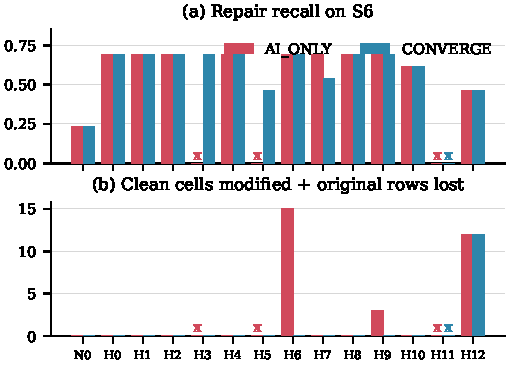
\includegraphics[width=\columnwidth]{injection.pdf}
\caption{E2 per-case outcomes on S6. An ``x'' marks an aborted run (no output).}
\label{fig:inject}
\end{figure}

The thirteen cases fall into five groups.

\noindent\textbf{(i) Caught by structure alone (H1, H2).} Invented and forbidden operation names are dropped by \textsc{AI\_Only}'s structural filter as well; both arms yield the oracle result. A closed operation catalog is, by itself, an effective first line of defence---an argument for recommendation over code generation.

\noindent\textbf{(ii) Availability failures prevented (H3, H5).} A phantom column or an out-of-domain parameter is caught by the executor's defence-in-depth checks under \textsc{AI\_Only}, but fail-fast semantics then \emph{abort the entire run}: one hallucinated recommendation discards every correct repair. \textsc{Converge} rejects the bad recommendation up front and executes the rest (H3: recall $0.69$; H5: $0.46$, since the substituted date operation is lost).

\noindent\textbf{(iii) Silent corruption prevented (H6, H9).} These are the most dangerous cases, because \textsc{AI\_Only} \emph{succeeds}. H6 smuggles an extra \texttt{sql} key into an otherwise valid \texttt{NORMALIZE\_CASE} on \texttt{city}; the executor ignores unknown keys, upper-cases the column, and damages 15 clean cells. H9 proposes \texttt{REMOVE\_DUPLICATES} on criteria \{\texttt{department}, \texttt{city}\}, which no evidence supports; \textsc{AI\_Only} silently deletes three \emph{original} employee records. \textsc{Converge} rejects both (unexpected parameter; no exact-criteria duplicate evidence) with zero damage.

\noindent\textbf{(iv) Conservativeness costs (H7, H8, H4).} H7 adds one fabricated key (\texttt{Engg.}) to an otherwise correct mapping. The fabricated key is harmless at execution time, so \textsc{AI\_Only} keeps all repairs (recall $0.69$), whereas \textsc{Converge} rejects the whole recommendation and loses two correct category repairs ($0.54$). This is the only case in which unvalidated AI outperforms validated AI. H8 (a contradicted null count) is rejected, leaving two salaries missing instead of incorrectly imputed: equal recall, but $2$ fewer incorrect repairs. H4 (trimming an integer column) is rejected on dtype but would have been a no-op.

\noindent\textbf{(v) Beyond the reach of validation (H10, H11, H12).} H10 maps the \emph{real} variant \texttt{mARKETING} to \texttt{Sales}. Every checkable predicate holds, the validator approves it, and both arms produce the same incorrect repair. H12 reproduces the evidence-type conflation observed in E1: whitespace evidence licenses a lowercase of \texttt{name}, which is approved and damages 12 clean cells in both arms. H11 proposes a constant \texttt{"unknown"} for an integer column; the parameter is a well-typed string, so the validator admits it at the \textsc{review} tier, and the executor's coercion check then aborts the run in \emph{both} arms. H11 identifies a concrete gap---type-coercibility of constant fill values is checkable from the profile and should be validated---whereas H10 is the irreducible class discussed in \S\ref{sec:discussion}.

\noindent\textbf{Summary.} Of the eleven checkable classes (H1--H9, H11, H12), the validator rejected nine. It turned two run aborts into successful partial cleaning and prevented 15 corrupted cells and 3 lost records. It cost two correct repairs in one case. The no-op control N0 (recall $0.23$) confirms that three whitespace repairs are performed by Spark's CSV writer irrespective of the plan.

\subsection{RQ4: Latency, Reliability, and Scalability}
\label{sec:res-scale}
\noindent\textbf{Latency.} In E1, \textsc{Spark\_Only} ran in $10$--$14$\,s per strategy invocation, while the AI arms took $105$--$295$\,s (Table~\ref{tab:main}). The difference is almost entirely model inference: the AI-analysis stage of \textsc{Converge} averaged $161\pm68$\,s per run (range $93$--$324$\,s) on the 4-core CPU, growing with the number of evidence items and hence with the length of the generated plan (S1, one item: $95$\,s; S6, five items: $278$\,s). Validation, including persistence of the audit record, took $61$--$130$\,ms per run, and the validator's checks alone take well under a millisecond (below). There is no systematic latency difference between \textsc{AI\_Only} and \textsc{Converge}; observed differences are within the run-to-run variation of CPU inference. The validation boundary is therefore effectively free relative to the model call.

\noindent\textbf{Reliability.} All 54 runs succeeded; schema-constrained decoding eliminated the parse failures and timeouts seen in the uncontrolled pilot. Recommendation consistency (mean pairwise Jaccard similarity of $(o,C_r)$ sets across repetitions) was $1.00$ on S1--S5 for both AI arms and $0.67$ on S6, where the model varied its plan (e.g., lowercasing \texttt{name} in some repetitions and \texttt{department} in another) even at temperature $0$. Temperature-$0$ decoding on quantised CPU inference is therefore not a reproducibility guarantee for multi-issue inputs, which strengthens the case for a deterministic gate.

\begin{figure}[t]
\centering
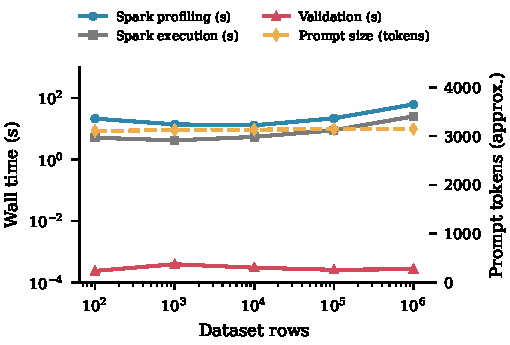
\includegraphics[width=\columnwidth]{scalability.pdf}
\caption{E3: Spark profiling and execution scale with data volume, whereas the AI-facing prompt and validation cost are independent of it (log--log; prompt size on the right axis).}
\label{fig:scale}
\end{figure}

\begin{table}[t]
\centering
\caption{E3 control-plane vs.\ data-plane cost by dataset size.}
\label{tab:scale}
\footnotesize
\setlength{\tabcolsep}{4pt}
\begin{tabular}{@{}rrrrrr@{}}
\toprule
\textbf{Rows} & \textbf{Profile (s)} & \textbf{Execute (s)} & \textbf{Prompt (chars)} & \textbf{Evid.} & \textbf{Validate (ms)}\\
\midrule
\tabinput{../tables/scalability.tex}
\bottomrule
\end{tabular}
\end{table}

\noindent\textbf{Scalability.} Fig.~\ref{fig:scale} and Table~\ref{tab:scale} report E3. Across four orders of magnitude ($10^2\to10^6$ rows, 6.4\,KB$\to$66\,MB), Spark profiling grew from $14$\,s to $62$\,s and plan execution from $4$\,s to $26$\,s (the $10^2$-row profiling time includes JVM warm-up). Over the same range the AI-facing prompt grew by only $1.4\%$ (12{,}423$\to$12{,}593 characters, $\approx$3.1k tokens; the growth is the extra digits in larger counts), the evidence bundle stayed at six items, and validating the six-recommendation plan took $0.24$--$0.40$\,ms regardless of size. This confirms the structural claim of \S\ref{sec:arch}: in CONVERGE the expensive, probabilistic component is invoked on $O(m+|E|)$ input, once per dataset, while the row-proportional work stays in the deterministic engine that was designed for it. A single model call of fixed cost can thus govern a cleaning job of arbitrary size, which is what makes LLM assistance economically compatible with big data workloads.


%======================================================================
\section{Discussion}
\label{sec:discussion}
%======================================================================
\subsection{What the Validation Boundary Buys}
The results support a nuanced reading of RQ2. The validator does not make the model \emph{smarter}: on the scenarios where the model's output was already correct, \textsc{AI\_Only} and \textsc{Converge} produce identical datasets. What the validator buys is a \emph{tighter worst case}. In E2, nine of eleven checkable hallucination classes were converted from potential data-integrity incidents (collateral modification, lost records, or an aborted run) into auditable rejections with a named rule, while the remaining correct recommendations still executed; in E1, the model's fabricated issues on S4 were rejected before they could corrupt 45 cells. This is precisely the property that big data operators require before delegating any decision to a component they cannot formally verify: for every hallucination class the validator can check, the blast radius of an error shrinks from \emph{doing the wrong thing at scale} to \emph{not doing} something---and the classes it cannot yet check are named and measured rather than unknown.

The audit trail matters as much as the verdict. Because every rejection records the rule that fired and the profiler fact it contradicted, operators can distinguish ``the model proposed something unsupported'' from ``the model misread a statistic'' from ``the model attempted a forbidden action''---three failure modes that warrant different responses (prompt revision, model replacement, and security review, respectively).

\subsection{What Validation Cannot Buy}
Two classes of error lie provably outside the reach of any evidence-based validator.

\emph{Semantically wrong but evidentially consistent recommendations} (H10) satisfy every checkable predicate of \S\ref{sec:problem}: the operation is legal, the column exists, the mapping key really occurs in the data. Only a judgement about the \emph{meaning} of ``Marketing'' versus ``Sales'' separates it from a correct repair. Such errors can be reduced but not eliminated by stronger structural rules---e.g., requiring every mapping to stay within one variant group (a normalisation-equivalence constraint), which would catch H10 specifically---or by consensus across models; ultimately they motivate the human approval boundary. The S3 behaviour in E1 is a natural instance: lowercasing \emph{does} unify the evidenced variants, and is rejected only by accident.

Two further gaps are \emph{not} fundamental and point to concrete fixes. Evidence-type conflation (H12, and the S6 approvals in E1) arises because the catalog lets one evidence type (\texttt{whitespace\_or\_casing}) license two semantically different operations; splitting the issue type, or requiring that a casing operation be justified by a variant group, closes it. The coercibility gap (H11) is closed by checking constant fill values against the column's semantic type. Likewise, the evidence-ambiguity defect found in the audit is fixed by accepting a claim if it matches \emph{any} candidate evidence item. All three are small, deterministic changes---the architecture makes such failures \emph{diagnosable and fixable}, which is itself a property unvalidated pipelines lack.

\emph{Information-theoretically unrecoverable repairs} are the second class. A missing salary cannot be restored to its true value from aggregate statistics; any imputation (mean, median, mode) is, by construction, an \emph{incorrect repair} under exact-match ground truth. S4's results should be read in this light: the correct behaviour for a cleaning system is not to maximise recall there, but to make the imputation explicit, reviewable, and reversible---which CONVERGE does by capping \texttt{FILL\_MISSING} at the \textsc{review} tier.

\subsection{The Conservativeness Cost}
Validation is not free. A single fabricated key in an otherwise-correct category mapping (H7) causes the \emph{entire} recommendation to be rejected, forfeiting its correct repairs. We consider this the right default for an unattended pipeline---partial trust in a recommendation whose evidence claims are known to be partly false is unjustified---but it suggests a refinement: \emph{repairable rejections}, in which the validator returns a minimally edited recommendation (here, the mapping with the fabricated key removed) for explicit approval. Similarly, short-circuiting on the first failing rule produces the most actionable explanation but hides additional violations; a ``report all'' mode would aid prompt engineering.

\subsection{Small Local Models as Recommenders}
The use of a 3B-parameter model quantised to 4 bits on a laptop CPU is deliberate. It reflects the deployment constraint that motivates CONVERGE in the first place---regulated data that may not leave the cluster---and it is the regime in which structured-output failures are most frequent. The architecture's value is largest exactly here: a weak model behind a strong validator is safe to deploy, whereas a strong model without one is merely \emph{usually} safe. Schema-constrained decoding was essential: in the earlier pilot without it, the same model returned \texttt{parameters} as a list and \texttt{evidence\_refs} as an object, failing strict parsing.

\subsection{Sink-Side Normalisation: A Methodological Lesson}
E2's no-op control revealed that Spark's CSV writer, with its default options, removes leading and trailing whitespace from every string field on output. Whitespace corruptions are therefore ``repaired'' by the storage layer regardless of the cleaning decision, and S1 cannot discriminate between arms. This is not an artefact of CONVERGE but of the execution substrate, and it generalises: when evaluating AI-assisted cleaning, the evaluator must include a no-op baseline to separate the effect of the decision layer from implicit normalisation in readers and writers. We report S1 for completeness and exclude it from comparative claims.

%======================================================================
\section{Threats to Validity}
\label{sec:threats}
%======================================================================
\noindent\textbf{Internal validity.} All arms share every component except the decision layer, and the evaluator is strategy-agnostic by construction (a test asserts it contains no strategy-specific branching). The approval policy is automated; a human approver could reject correct recommendations or accept wrong ones. Temperature-$0$ decoding reduces but does not remove stochasticity under quantised CPU inference.

\noindent\textbf{Construct validity.} Exact-match ground truth penalises semantically acceptable alternatives (e.g., a different but reasonable imputation). Before/after issue counts are reported separately precisely because they measure \emph{absence of detected issues}, not correctness. Repair precision is not observable and is not reported.

\noindent\textbf{External validity.} The reference table has 15 rows and 7 columns and covers five corruption types; real datasets exhibit richer errors (functional-dependency violations, cross-column inconsistencies, typos). We evaluated one local model; larger or remote models (e.g., Gemini, supported by the implementation) may differ in recall and failure profile. Spark ran in \texttt{local[*]} mode; the control-plane scalability result (E3) is structural, but absolute Spark timings on a cluster will differ.

\noindent\textbf{Conclusion validity.} With three repetitions per cell we report means and standard deviations but do not claim statistical significance; the E2 study is deterministic and its conclusions do not depend on sampling.

%======================================================================
\section{Future Directions}
\label{sec:future}
%======================================================================
Our results suggest that the most productive path for integrating generative AI with traditional big data pipelines is not to make models execute, but to make their proposals \emph{verifiable}. We highlight seven directions.

\begin{enumerate}[leftmargin=*,nosep]
  \item \textbf{Richer evidence languages.} Extending the profiler to emit functional-dependency, cross-column, and distributional-drift evidence (in the spirit of Deequ~\cite{schelter2018deequ} and CFDs~\cite{fan2008cfd}) would let the catalog grow while keeping every operation checkable.
  \item \textbf{Semantic validators.} Normalisation-equivalence constraints, reference-vocabulary lookups, and multi-model agreement can narrow the H10 gap without surrendering determinism.
  \item \textbf{Repairable rejections and dialogue.} Feeding validator explanations back to the model, Reflexion-style~\cite{shinn2023reflexion}, turns rejections into a bounded self-correction loop whose output is \emph{re-validated}, preserving complete mediation.
  \item \textbf{Placement beyond cleaning.} The same recommend--validate--execute pattern applies before ingestion (schema inference), during processing (partitioning and join-order hints validated against cost models), and after processing (natural-language insights validated against computed aggregates).
  \item \textbf{Cluster-scale evaluation.} Because the prompt is $O(m+|E|)$, a single model call can govern a petabyte-scale Spark job; the open question is how to sample and bound evidence for very wide or high-cardinality schemas.
  \item \textbf{Cost and carbon accounting.} Exposing token usage through the provider interface would allow cost-aware placement between local SLMs and remote LLMs, guided by scaling behaviour~\cite{kaplan2020scaling}.
  \item \textbf{Adversarial robustness.} Evidence contains raw cell values; a malicious cell could attempt indirect prompt injection~\cite{greshake2023injection}. Because the validator treats all output as untrusted, the architecture already bounds the damage, but systematic red-teaming of the evidence channel is needed.
\end{enumerate}

%======================================================================
\section{Conclusion}
\label{sec:conclusion}
%======================================================================
We presented CONVERGE, a validation-guided architecture for integrating language models into Spark data-cleaning pipelines, in which the model recommends, an independent deterministic validator decides against Spark-computed evidence, and Spark executes an immutable, fail-fast plan. Under controlled, ground-truth conditions with a local 3B-parameter model, AI-assisted cleaning repaired a corruption class that a principled deterministic baseline must leave untouched (mixed date formats, recall $0\to1$), but unvalidated AI also fabricated issues and destroyed up to 45 clean cells in a single run---damage that standard before/after quality checks scored as a success. The validation boundary cut collateral damage by 71--88\%, rejected nine of the eleven checkable hallucination classes we injected---turning silent corruption, deleted records and aborted runs into auditable rejections---and did so at a sub-millisecond control-plane cost that does not grow with data volume. Validation is not a substitute for semantic correctness: semantically wrong but evidentially consistent recommendations, catalog-level evidence conflation, and unrecoverable imputations remain, and they define where human review and future semantic validators must focus. The broader lesson for the future of big data systems is architectural: generative models are most valuable to traditional pipelines when they are confined to proposing, and every proposal is checked by the deterministic machinery those pipelines already trust.

\section*{Artifact Availability}
The CONVERGE implementation, controlled-corruption generator, ground-truth manifests, experiment harness, raw per-run results, and the scripts that produced every figure and table in this paper are contained in the project repository (\texttt{src/converge}, \texttt{experiments/}, \texttt{paper/scripts/}). All 510 automated tests pass.


\bibliographystyle{IEEEtran}
\bibliography{refs}

\end{document}
